\subsection{Numeric strings}
\label{subsec:pd:numericstrings}


% ----------------------- paths to graphics ------------------------

\graphicspath{{5_automatic_learning/pattern_detection/images/}}

% ----------------------- contents from here ------------------------
% 

This pattern detector searches for numbers stored in string columns. Once found, it changes the column data type to a numeric one, while also preserving the string format of the numbers in additional columns. The purpose is to optimize the data type and create opportunities for numeric compression schemes. The \textit{select\_column} method only returns \textit{True} for \verb|VARCHAR| columns. This is a single-column pattern detector and columns are evaluated independently. The next paragraphs describe the pattern detection process for a single column.

The \textit{scanning} phase checks for each value (\(v_{string}\)) whether it can be parsed as a number (\(v_{numeric}\)). If \textit{True}, it extracts the format information and checks whether the original string value can be reconstructed. The \textit{evaluation} phase chooses an appropriate numeric data type (e.g. \verb|DECIMAL(p,s)|) based on the type and range of the values selected in the \textit{scanning} phase. More details about the format preserving and data type inference processes are presented in the following paragraphs.

\textbf{Format preserving.} While analyzing the Public BI benchmark we noticed that the majority of string values \(v_{string}\) with a different format than their numeric representation \(v_{numeric}\) contain leading or trailing characters (e.g. zeros, whitespace). Therefore, we based our format preserving technique on 3 components---\textit{prefix}, \(v_{numeric}\), \textit{suffix}---as follows:\\
Step-1: cast \(v_{string}\) to number to obtain \(v_{numeric}\)\\
Step-2: check whether \(abs(v_{numeric})\) is a substring of \(v_{string}\). If \textit{False}, the format cannot be preserved. Otherwise, \(v_{string}\) has the following format:
\verb|${|\textit{prefix}\verb|}|\(abs(v_{numeric})\)\verb|${|\textit{suffix}\verb|}|,
where \textit{prefix} and \textit{suffix} can be any strings, including the empty string.\\
Step-3: extract the \textit{prefix} and \textit{suffix} and store them as format information together with \(v_{numeric}\).

\(v_{string}\) can be now reconstructed by concatenating the \textit{prefix}, \(v_{numeric}\) and \textit{suffix} values. Table~\ref{tab:pd:numericstring:formatexamples} illustrates a few examples that the format preserving technique covers (\verb|"_"| characters represent spaces).

\begin{table}[h]
\centering
\begin{tabular}{@{}llllll@{}}
\toprule
\(v_{string}\)    & \(v_{numeric}\) & \textit{prefix} & \(abs(v_{numeric})\) & \textit{suffix} & \textit{description}               \\ \midrule
\verb|"1.23"|     & \verb|1.23|     & \verb|""|       & \verb|1.23|          & \verb|""|       & no format information              \\
\verb|"1.2300"|   & \verb|1.23|     & \verb|""|       & \verb|1.23|          & \verb|"00"|     & trailing zeros                     \\
\verb|"000.1"|    & \verb|0.1|      & \verb|"00"|     & \verb|0.1|           & \verb|""|       & leading zeros                      \\
\verb|"+10"|      & \verb|10|       & \verb|"+"|      & \verb|10|            & \verb|""|       & \(+\) sign                         \\
\verb|"-10"|      & \verb|-10|      & \verb|"-"|      & \verb|10|            & \verb|""|       & negative number                    \\
\verb|"-000.5"|   & \verb|-0.5|     & \verb|"-00"|    & \verb|0.5|           & \verb|""|       & negative number with leading zeros \\
\verb|"__54\t\t"| & \verb|54|       & \verb|"__"|     & \verb|54|            & \verb|"\t\t"|   & leading and trailing whitespace    \\ \bottomrule
\end{tabular}
\caption{Numeric string format preserving examples}
\label{tab:pd:numericstring:formatexamples}
\end{table}

We do not support---and consider exceptions---the following: 1) numbers in scientific notation; 2) other notations or abbreviations (e.g. \verb|.12| instead of \verb|0.12|, \verb|1_000_000| instead of \verb|1000000|, etc.).

\textbf{Data type inference.} The purpose of this pattern detector is to store the numeric string values in a numeric column, which requires a numeric data type. We chose two data types that can be used to represent all numbers: \verb|DECIMAL(p,s)| and \verb|DOUBLE|. During the \textit{scanning} phase all \(v_{numeric}\) values are interpreted as decimals. The maximum number of digits before and after the decimal point---\(\mathit{integer}_{dmax}\) and \(\mathit{fractional}_{dmax}\)---are determined.  In the \textit{evaluation} phase, the parameters \textit{p} (precision) and \textit{s} (scale) of the \verb|DECIMAL(p,s)| data type are computed as follows:
\begin{equation}
\label{eq:pd:numericstrings:precisionscale}
\begin{array}{ll}
    p &= \mathit{integer}_{dmax} + \mathit{fractional}_{dmax}\\
    s &= \mathit{fractional}_{dmax}
\end{array}
\end{equation}
The final datatype of the numeric column is determined as follows:
\begin{equation}
\label{eq:pd:numericstrings:datatype}
\mathit{datatype} = 
\left\{
\begin{array}{ll}
    \verb|DECIMAL(p,s)| & \mbox{if } p \leq p_{max}\\
    \verb|DOUBLE| & \mbox{else}
\end{array}
\right.
\end{equation}
where:
\begin{itemize}
    \item[] \(p_{max}\) = maximum decimal precision supported by the system
\end{itemize}
The maximum precision value is configurable and necessary as database systems enforce it---MonetDB: \(p_{max}=38\) \cite{monetdbdatatypes}, VectorWise: \(p_{max}=39\) \cite{vectorwisedecimal}.

A string value \(v_{string}\) is considered an exception if any of the following conditions is not satisfied:\\
1) \(v_{string}\) cannot be parsed as a numeric value \(v_{numeric}\)\\
2) \(v_{string}\) cannot be reconstructed from its numeric value \(v_{numeric}\) and format information\\
3) \(v_{numeric}\) exceeds the numeric data type selected in the \textit{evaluation} phase

There is no strict filtering condition that determines whether a column fits this pattern or not. The pattern detector outputs a result for all columns with \textit{coverage} grater than \(0\), leaving the responsibility of choosing which columns to compress with this scheme to the compression learning algorithm. The \textit{evaluation result} is composed of the \textit{coverage} and \textit{row\_mask}---as defined in \ref{subsec:genericpd}~\nameref{subsec:genericpd}. No additional metadata is necessary for the compression and decompression processes.

The \textit{expression nodes} for the \nameref{subsec:pd:numericstrings} pattern are illustrated in the Figure~\ref{fig:pd:numericstrings:exprnode}.

\begin{figure}[h]
  \centering
  \begin{subfigure}[t]{0.49\linewidth}
    \centering
    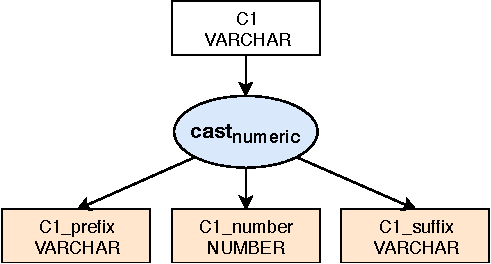
\includegraphics[width=1\linewidth]{expression_node-nas-compression_3.pdf}
    \caption[b]{compression}
    \label{fig:pd:numericstrings:exprnode:compression}
  \end{subfigure}
%   \hspace{1em}
  \begin{subfigure}[t]{0.49\linewidth}
    \centering
    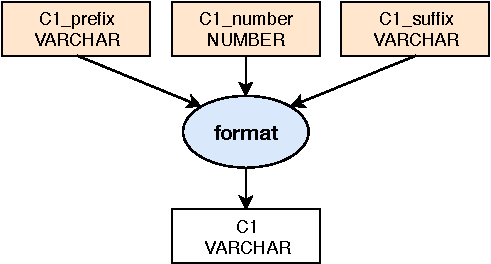
\includegraphics[width=1\linewidth]{expression_node-nas-decompression_3.pdf}
    \caption[b]{decompression}
    \label{fig:pd:numericstrings:exprnode:decompression}
  \end{subfigure}
  \caption{Numeric strings expression nodes}
  \label{fig:pd:numericstrings:exprnode}
\end{figure}

The \textit{compression node} takes as input the \textit{string} column and generates three output columns: one for storing the numeric values and the other two for storing the format information as \textit{prefix} and \textit{suffix}. The \textit{decompression node} takes as input the \textit{numeric}, \textit{prefix} and \textit{suffix} columns and reconstructs the original string column.

The compression operator \(cast_{numeric}\) takes as input \(v_{string}\) and tries to represent it as the 3 components---\textit{prefix}, \(v_{numeric}\) and \textit{suffix}---as described above. It then checks whether \(v_{numeric}\) fits in the inferred data type of the numeric column. If everything succeeds it returns the 3 values, else it raises an \textit{OperatorException} indicating that \(v_{string}\) should be added to the exception column. The decompression operator \(concat\) reconstructs \(v_{string}\) by concatenating \textit{prefix}, \(abs(v_{numeric})\) and \textit{suffix}. The two operators do not require any metadata, except for the numeric column data type.

There are two main benefits brought by this representation scheme: 1) using an optimal numeric data type instead of \verb|VARCHAR|, leading to smaller size on disk; 2) creating opportunities to further compress the numeric column with numeric compression schemes. Moreover, we noticed that in practice the \textit{prefix} and \textit{suffix} columns get further compressed as \nameref{subsec:pd:constant} or with \nameref{subsec:pd:dict} encoding.

% ---------------------------------------------------------------------------
% ----------------------- end of thesis sub-document ------------------------
% ---------------------------------------------------------------------------